\documentclass[tikz, border=12pt]{standalone}
\usepackage{tikz}
\usetikzlibrary{decorations.pathreplacing}

\begin{document}

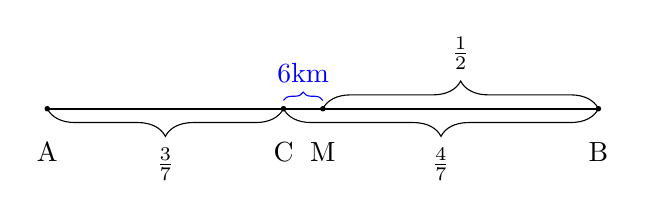
\begin{tikzpicture}
	\coordinate (A) at (0,0);
	\coordinate (C) at (3,0);
	\coordinate (M) at (3.5,0);
	\coordinate (B) at (7,0);
    % 绘制主要的线段AB
    \draw[thick] (A) -- (B);
    
    % 添加实心圆点标注A、B、C、M、D
    \fill (A) circle (1pt) node[below=3mm] {A};
    \fill (B) circle (1pt) node[below=3mm] {B};
    \fill (C) circle (1pt) node[below=3mm] {C};
    \fill (M) circle (1pt) node[below=3mm] {M};
    
    % 添加距离比例3:4的标注(尖头朝下)
    \draw [decorate,decoration={brace,amplitude=10pt,mirror},yshift=-10pt]
        (A) -- (C) node [black,midway,yshift=-20pt] {$\frac{3}{7}$};
        
    \draw [decorate,decoration={brace,amplitude=10pt,mirror},yshift=-10pt]
        (C) -- (B) node [black,midway,yshift=-20pt] {$\frac{4}{7}$};
    
    \draw [decorate,decoration={brace,amplitude=10pt},yshift=10pt]
        (M) -- (B) node [black,midway,yshift=20pt] {$\frac{1}{2}$};
        
    % 添加点M到C的距离6km的标注(尖头朝上)
    \draw [blue,decorate,decoration={brace,amplitude=3pt},yshift=3pt]
        (3,0) -- (3.5,0) node [blue,midway,yshift=10pt] {6km};
    
\end{tikzpicture}

\end{document}